%% Example of a LaTeX source file for a COLING-2012 submission
%% last updated: July 10, 2012
\documentclass[10pt,a5paper,twoside]{article}
\usepackage{coling2012}
\usepackage{booktabs}
%\usepackage{times}
\usepackage{multirow}
\usepackage{alltt}
\usepackage[small,bf]{caption}

\newcommand{\tag}[1]{{\small{\texttt{#1}}}}

\title{Rule-based Machine Translation between Indonesian and Malaysian}
%\author{$Author^{1}$ \\
%{\small  	(1) Affiliation\\
%  \texttt{author@affiliation} \\ 
%}}


\author{$Raymond~Hendy~Susanto^{1}$
    $Septina~Dian~Larasati^{2}$
    $Francis~M.~Tyers^{3}$ \\
{\small  	(1) Department of Computer Science, National University of Singapore\\
(2) Institute of Formal and Applied Linguistics, MFF, Charles University in Prague\\
(3) Dept. Lleng. i Sist. Inform., Universitat d’Alacant\\
  \texttt{raymondhs@nus.edu.sg}, \texttt{larasati@ufal.mff.cuni.cz}, \texttt{ftyers@dlsi.ua.es}\\ 
}}

\begin{document}
\maketitle

\abstractEn{
We describe the development of a bidirectional rule-based machine translation system between Indonesian and Malaysian (id-ms), two closely related Austronesian languages natively spoken by approximately 35 million people. The system is based on the re-use of free and publicly available resources, such as the Apertium machine translation platform and Wikipedia articles. We also present our approaches to overcome the data scarcity problems in both languages by exploiting the morphology similarities between the two.}

\keywordsEn{machine translation, Malay languages, morphology}

\newpage
\section{Introduction}
In this paper we describe the development of \texttt{\small{apertium-id-ms}}, a bidirectional Indonesian and Malaysian machine translation system based on the Apertium platform. The paper is laid out as follows: Section~\ref{sec:lang} gives a brief description of the two languages; Section~\ref{sec:prev} gives a short review of the previous work in Indonesian-Malaysian language pair; Section~\ref{sec:sys} describes the system and the creation of the resources; Section~\ref{sec:eval} presents an evaluation of the system, and finally we describes future work that could be done and some concluding remarks.

\section{Languages}
\label{sec:lang}
Indonesian (\emph{Bahasa Indonesia}) and Malaysian (\emph{Bahasa Malaysia}) are standards of the Malay language and both belong to the Austronesian family. Indonesian is spoken by approximately 35 million people\footnote{\url{http://www.lmp.ucla.edu/Profile.aspx?menu=004&LangID=89} Last accessed: October 2012}, mostly from Indonesia, but also widespread in the Netherlands, the Philippines, Saudi Arabia, Singapore, and the United States. Malaysian has 10 million speakers across the Peninsular Malaysia, and other speakers coming from parts of Sarawak, Indonesia (Sumatra), Singapore, and United States.

Indonesian and Malaysian are closely related; both languages are mutually intelligible to a great extent. The morphology of the two languages are the same, where agglutination is used extensively (by means of affixation, reduplication, and compounding), although some affixes are more frequently used in one language over the other. For instance, the prefix \emph{juru-} is often used in Malaysian to indicate an actor characterized by the stem it is attached to. While this affixation also happens in Indonesian, it is not as frequently found as in Malaysian.

The main difference between Indonesian and Malaysian languages lies in their vocabulary; Indonesian is largely influenced by Dutch and Javanese, whereas Malaysian has many words borrowed from English, e.g. \emph{dokter} vs. \emph{doktor} (`doctor') and \emph{tas} vs. \emph{beg} (`bag'). Moreover, there are frequent minor spelling differences, e.g. \emph{kabar} vs. \emph{khabar} (`news') and \emph{mau} vs. \emph{mahu} (`want').

%\section{Previous work}
\section{Motivation}
\label{sec:prev}
The development of this system is motivated by an early prototype Apertium system developed in \citet{larasati2010study}. Since then, most of the components in the prototype were completely redesigned, and the direction of the development was based on the following rationale:
\begin{itemize}
\item{Morphological analyser: We wanted to create a morphological analyser which is not only robust, but also does not overgenerate either. Both Indonesian and Malaysian morphology are characterized by rich derivational morphology, but poor inflectional morphology, unlike some other morphologically-complex languages such as Arabic and Turkish. Moreover, each root undergoes an idiosyncratic subset of these derivational processes (i.e. we cannot simply apply the derivational affixes to new words).}
\item{Bidirectional: A new translation direction from Malaysian to Indonesian was added, and used as the starting point instead of the opposite direction, since translating from Indonesian to Malaysian appears to be more ambiguous.}
\item{Evaluation: Finally, we performed a quality evaluation of our system, which has not been done before.}
\end{itemize}
%Furthermore, there exists a statistical machine translation system that has been developed for this language pair, that is Google Translate\footnote{\url{http://translate.google.com/}}, a web-based multilingual translation system.

We have chosen the rule-based approach, instead of the ubiquitous corpus-based statistical approach, due to the dearth of parallel corpora for the two languages. Moreover, the closeness between the two languages makes the rule-based approach favourable. Recent development for closely related languages with the rule-based approach have shown competitive performance with respect to the statistical approach, e.g. the rule-based Swedish$\rightarrow$Danish system in \citet{tyers2009svda} and the Italian$\rightarrow$Catalan system in \citet{tyers2011itca}, where both systems outperform a rivaling statistical-based system.

\section{System}
\label{sec:sys}
The system is based on the Apertium machine translation platform \citep{apertium/2011}.\footnote{\url{http://www.apertium.org/}} The platform was originally aimed at the Romance languages of the Iberian peninsula, but has also been adapted for other, more distantly related language pairs. The whole platform, both programs and data, are licensed under the Free Software Foundation's General Public Licence\footnote{\url{http://www.fsf.org/licensing/licenses/gpl.html}} (GPL) and all the software and data for the 33 supported language pairs (and the other pairs being worked on) is available for download from the project website.

\subsection{Architecture of the system}

\begin{figure*}[htbp]
\begin{center}
 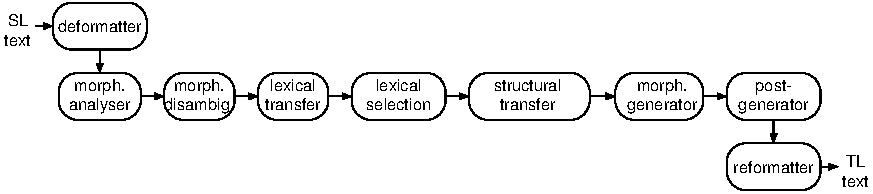
\includegraphics[width=0.8\textwidth]{architecture.pdf}
\end{center}
\caption{The pipeline architecture of the Apertium system.}
\label{fig:modules}
\end{figure*}

The Apertium translation engine consists of a Unix-style \emph{pipeline} or
\emph{assembly line} with the following modules (see Fig.~\ref{fig:modules}):  
\begin{itemize}
\item A \emph{deformatter} which encapsulates the format information
 in the input as \emph{superblanks} that will then be seen
 as blanks between words by the other modules.
\item A \emph{morphological analyser} which segments the text in
  surface forms (SF) (\emph{words}, or, where detected, multi-word lexical
  units or MWLUs) and for each, delivers one or more \emph{lexical
    forms} (LF) consisting of \emph{lemma}, \emph{lexical category} and
  morphological information. 
\item A \emph{morphological disambiguator} (constraint grammar) which chooses, using linguistic rules
  the most adequate sequence of morphological analyses for an ambiguous sentence. 
\item A \emph{lexical transfer} module which reads each SL LF 
  and delivers the corresponding target-language (TL) LF
  by looking it up in a bilingual dictionary encoded as an FST
  compiled from the corresponding XML file. The lexical transfer module may
  return more than one TL LF for a single SL LF.
\item A \emph{lexical selection} module which chooses, based on context 
  rules the most adequate translation of ambiguous source language LFs.
\item A \emph{structural transfer} module which
    performs local syntactic operations, is compiled from XML files containing rules that 
    associate an \emph{action} to each defined LF \emph{pattern}. Patterns are applied left-to-right, and the 
    longest matching pattern is always selected.
\item A \emph{morphological generator} which delivers a TL SF
 for each TL LF, by suitably inflecting it. 
\item A \emph{reformatter} which de-encapsulates any format
  information.
\end{itemize}

\subsection{Morphological transducers}
There is one publicly available morphological tool for Indonesian, MorphInd \citep{larasati2011indonesian}. However, MorphInd is only designed for analysis, while we wanted a tool for both morphological analysis and generation. Moreover, there are rarely linguistic resources and tools available for Malaysian. \citet{Baldwin06opensource} has developed the free/open-source lemmatiser for Malay, but this does not meet our need either since we wanted to include more robust morphological information into our Malaysian transducer, such as part-of-speech and affixes. Thus, we decided to build the morphological transducers from scratch.

Similar to most Apertium language pairs, the morphological transducers for both Indonesian and Malaysian are constructed using \emph{lttoolbox}, a toolbox for morphological analysis and generation that is available under a free/open-source licence. The monolingual dictionary for each language is provided as XML-formatted entries, which is then compiled into a finite state transducers using \emph{lttoolbox}.

\subsubsection{Indonesian morphological transducer}
A lexicon list was created semi-automatically to the Indonesian morphological analyser based on a words frequency list, with the most frequent words being added first. The frequency list was taken from a database dump of the Indonesian Wikipedia. For each word in the frequency list, we obtained its lemma and part-of-speech information from Kateglo\footnote{\url{http://kateglo.bahtera.org/}}, an online Indonesian dictionary with over 70,000 entries licensed under CC BY-SA 3.0.\footnote{\url{http://creativecommonsorg/licenses/by-sa/3.0/}}. Since we also wanted to include affix information in our analyser, we wrote a rule-based morpheme segmentor to decompose a given Indonesian surface form into their constituent morphemes, also by making use of the lemma information from Kateglo. Moreover, closed word classes (e.g. pronouns, conjunctions) were added by hand.

\subsubsection{Malaysian morphological transducer}
A frequency list for Malaysian was also created based on a database dump of the Malaysian Wikipedia. Unlike Indonesian, we did not find a comprehensive Malaysian dictionary with adequate morphological information, such as lemma and part-of-speech. Hence, the Malaysian analyser was built using the two strategies below.

First, Malaysian words that also exist as an Indonesian word were assumed to share the same morphological information (i.e. the same lemma and part-of-speech), and were added automatically to the analyser. Although this method may introduce a number of false friends (e.g. \emph{polisi} means `policy' in Malay but `police' in Indonesian), the benefit outweighs the risk since there is huge overlap in the lexicons of the two languages. Moreover, most of these false friends usually belong to the same part-of-speech.

Second, we also added Malaysian words which appear in our bilingual dictionary. Since every entry in a bilingual dictionary is a pair of words with the same meaning, we can assume that these words also belong to the same part-of-speech most of the time. Our approaches to building the bilingual dictionary are presented in the following section.

\subsection{Bilingual dictionary}

% \begin{figure*}[htbp]
% \begin{center}
% \begin{small}
% \begin{alltt}
% <e><p><l>\textbf{mobil}<s n="n"/></l><r>\textbf{kereta}<s n="n"/></r></p></e>
% <e><p><l>\textbf{mobilitas}<s n="n"/></l><r>\textbf{mobiliti}<s n="n"/></r></p></e>
% <e><p><l>\textbf{sepeda}<s n="n"/></l><r>\textbf{basikal}<s n="n"/></r></p></e>
% <e><p><l>\textbf{modern}<s n="adj"/></l><r>\textbf{moden}<s n="adj"/></r></p></e>
% <e><p><l>\textbf{karena}<s n="cnjsub"/></l><r>\textbf{kerana}<s n="cnjsub"/></r></p></e>
% \end{alltt}
% \end{small}
% \caption{Example entries from the bilingual dictionary. Indonesian is on the left, and Malaysian on the right.}
% \label{fig:bidix}
% \end{center}
% %\vspace{-1em}
% \end{figure*}

There is no freely available bilingual dictionary between Indonesian and Malaysian, so we had to build the dictionary from scratch. At the moment, the bilingual dictionary contains 12,142 entries, which was developed in several ways described below.

First, most of the entries were added using automatic word alignments. We created an Indonesian-Malaysian parallel corpus by translating many articles taken from Malaysian Wikipedia. The translation process is mostly automatic, with the help of existing Malaysian-Indonesian machine translation systems such as Google Translate.\footnote{\url{http://translate.google.com/}}

Next the Wikipedia corpus is tagged using our morphological analyser, and word alignments were created by running \texttt{GIZA++} \citep{Och2003align} on the tagged corpus. We fed the probabilistic dictionary into the \texttt{ReTraTos} toolbox \citep{Caseli2006retratos}, which extracts both phrases and single-word translations from alignments, and converts them into Apertium translation entries. The \texttt{ReTraTos} method gave us about 12,000 translation entries, but also required a manual check due the amount of noise in the resulting data.

Finally, some entries were added manually, which included closed word classes and words that frequently appeared in Wikipedia but were not yet added to the bilingual dictionary.

\subsection{Disambiguation}
The output from the morphological analysis is disambiguated using Apertium's statistical disambiguator module. The module implements a bigram part-of-speech tagger based on hidden Markov models (HMM). To improve the accuracy of our disambiguator, a Constraint Grammar \citep{Karlsson1990cg} could be used as a pre-disambiguator module before feeding the input to the HMM, which is left for future work.

\subsection{Lexical selection rules}
Given the closeness of the languages, lexical selection is not a large problem between Indonesian and Malaysian. However, a number of rules can be written for ambiguous words; for example, the Malaysian preposition \emph{daripada} `from (to explain the origin of something), than (comparison)' can be translated into Indonesian as either \emph{dari} `from' or \emph{daripada} `than (comparison)', depending on the surrounding context.

Another example is the copulas \emph{adalah} and \emph{ialah} (both meaning `be'), which exist in both Indonesian and Malaysian, but have a slightly different usage in each language. In Malaysian, \emph{adalah} is used before an adjective phrase or a prepositional phrase, and \emph{ialah} is used only before a noun phrase. In comparison to Indonesian, there are no strict rules governing the use of the two words, and their usage is more interchangeable.
\subsection{Transfer rules}
There are barely differences between the grammar of Indonesian and Malaysian, in that the structure of words, phrases, clauses, and sentences are almost exactly the same. That said, the lexical transfer between the two languages works by simple word substitution in most cases.

\begin{table*}[htbp]
\centering
\begin{tabular}{ll}
%\hline
%{\bf Stage} & {\bf Representation} \\
\toprule
{\bf (Malaysian) Input} & Cuaca kelmarin amatlah sejuk. \\ 
\midrule
%^Cuaca/Cuaca<n><sg>$ ^kelmarin/kelmarin<adv>$ ^amatlah/amatlah<adv>$ ^sejuk/sejuk<adj>$^./.<sent>$^./.<sent>$
{\bf Mor. analysis} & \^{}Cuaca/Cuaca\tag{<n>}\tag{<sg>\$} \^{}kelmarin/kelmarin\tag{<adv>\$}\\
~ & \^{}amatlah/amatlah\tag{<adv>\$} \^{}sejuk/sejuk\tag{<adj>\$}\\
~ & \^{}./.\tag{<sent>\$}\\
\midrule
% ^Cuaca<n><sg>$ ^kelmarin<adv>$ ^amatlah<adv>$ ^sejuk<adj>$^.<sent>$^.<sent>$
{\bf Mor. disambiguation}& \^{}Cuaca\tag{<n>}\tag{<sg>\$} \^{}kelmarin\tag{<adv>\$} \^{}amatlah\tag{<adv>\$}\\
~ & \^{}sejuk\tag{<adj>\$}\^{}.\tag{<sent>\$} \\
\midrule
% ^Cuaca<n><sg>$ ^kemarin<adv>$ ^amatlah<adv>$ ^dingin<adj>$^.<sent>$^.<sent>$
{\bf Transfer}& \^{}Cuaca\tag{<n>}\tag{<sg>\$} \^{}kemarin\tag{<adv>\$} \^{}amatlah\tag{<adv>\$}\\
~ & \^{}dingin\tag{<adj>\$}\^{}.\tag{<sent>\$} \\ 
\midrule
{\bf Mor. generation} & Cuaca kemarin amatlah dingin. \\
\bottomrule
\end{tabular}
 \caption{Translation process for the sentence \emph{Cuaca kelmarin amatlah sejuk.} `The weather yesterday is very cold'.}
\end{table*}

\section{Evaluation}
\label{sec:eval}
The system was evaluated in three ways. The first was the coverage\footnote{Here coverage is defined as \emph{na\"ive coverage}, that is for any given surface form at least one analysis is returned by our monolingual dictionaries} of the system. The second was the word error rate (WER) of the translation output for our test data set, together with the error analysis of the translations. Lastly, we did a comparative evaluation with an existing system.

\subsection{Coverage}
Lexical coverage of the system is calculated over the Indonesian and Malaysian Wikipedia articles, as shown in Table~\ref{table:coverage}. The database dump of the Indonesian Wikipedia\footnote{\url{http://id.wikipedia.org/}; \texttt{idwiki-20120429-pages-articles.xml.bz2}} was from the 29th April 2012, and that of Malaysian Wikipedia\footnote{\url{http://ms.wikipedia.org/}; \texttt{mswiki-20120428-pages-articles.xml.bz2}} from the 28th April 2012. Both database dumps were stripped of formatting.

\begin{table}[htbp]
  \begin{center}
  \begin{tabular}{ccc}
  \toprule
  \bf{Corpus} & \bf{Tokens} & \bf{Coverage}\\
  \midrule
  Indonesian Wikipedia & 19,021,087 & 80.70\% \\
  \midrule
  Malaysian Wikipedia & 12,613,364 & 80.10\% \\
  \bottomrule
  \end{tabular}
  \caption{Na\"ive vocabulary coverage over Wikipedia articles.}
  \label{table:coverage}
  \end{center}
\end{table}

\subsection{Quantitative and Qualitative}
We tested our system on a 2,084 word text taken from various articles in Malaysian Wikipedia. The translation quality was measured using Word Error Rate (WER), a metric based on the Levenshtein distance \citep{levenshtein/1966}. We calculated the WER for each sentence using the \texttt{\small{apertium-eval-translator}}\footnote{\url{https://apertium.svn.sourceforge.net/svnroot/apertium/trunk/apertium-eval-translator/}} tool. The WER metric was preferred to other MT metrics such as BLEU \citep{Papineni2002bleu} since we want to evaluate the system for the \emph{postedition} task. That is, we want to assess the amount of manual labour needed to improve the machine-generated translation.\footnote{BLEU is not used in our evaluation because we are using a reference translation which is a postedition of the machine-translated text, and the normal use of BLEU is for evaluating against a non-postedited reference. If we used BLEU it would give artifically high scores.}

For the Malaysian to Indonesian direction, the sentences were translated by the system, and then postedited by a native Indonesian speaker. For the Indonesian to Malaysian direction, we used the reference translation, as postedited by the native speaker and used it as a source of Indonesian to be translated to Malaysian, then the original Malaysian sentence was used as the reference translation.

\begin{table}[htbp]
  \begin{center}
  \begin{tabular}{ccccr}
  \toprule
  \bf{Corpus}                 & \bf{Direction}         & \bf{Tokens}  & \bf{Unknown} & \multicolumn{1}{c}{\bf{WER}}  \\
  \midrule
  \multirow{2}{*}{Malaysian Wikipedia} & id$\rightarrow$ms & 2,079     & 211  & 14.43\% (83.89\%) \\
                          & ms$\rightarrow$id & 2,084     & 256  & 7.58\% (69.53\%)  \\
  \bottomrule
  \end{tabular}
    \caption{Word error rate over the Malaysian Wikipedia test data. Number in parentheses gives percentage of unknown words which were free rides.}
    \label{table:wer}
  \end{center}
\end{table}

We consider the WER of our system, as depicted in Table~\ref{table:wer} is quite acceptable for postediting. In our system, unknown words are left unprocessed. Nonetheless, many of these unknown words are \emph{free rides}\footnote{That is, the word is unknown to the system, but the same in Indonesian and Malaysian. Typical free-rides include names and special terminology.}, which will not affect the final quality of the translation.

As a direction for future improvement, we did an error analysis by reviewing the translation outputs from our system. Most of the translation errors were due to the mistakes and gaps in our analyser. Specifically, many of the stems do not have the complete set of its derived forms. As a result, it cannot provide analysis for a unknown derived wordform even if the stem already exists in the analyser. Moreover, the analyser cannot handle clitics attached to unknown words (e.g. possessive enclitic \emph{-nya}). These errors can be fixed by a more thorough revision of the morphological analyser. Lastly, the system is often not capable of choosing the most suitable translation given a particular context. A lexical selection module can be written to alleviate this problem.
\begin{table}[htbp]
  \begin{center}
  \begin{tabular}{clr}
  \toprule
  \bf{Dir.}                 & \bf{System}         & \multicolumn{1}{c}{\bf{WER}}  \\
  \midrule
  \multirow{2}{*}{id$\rightarrow$ms} & Apertium & 14.43\% \\
                                     & Google & 13.90\% \\
  \midrule
  \multirow{2}{*}{ms$\rightarrow$id} & Apertium & 7.58\% \\
                                     & Google & 4.07\% \\
  \bottomrule
  \end{tabular}
    \caption{Accuracy comparison between the two systems.}
    \label{table:comp}
  \end{center}
\end{table}

\subsection{Comparative}
We compared our system to another MT system for Indonesian to Malaysian and Malaysian to Indonesian, Google Translate, a web-based statistical machine translation system. The evaluation was performed the same way: the test data was translated with Google Translate, then postedited.

We notice from Table~\ref{table:comp} that Google outperforms the Apertium system in both translation directions. For Malaysian to Indonesian, the error rate is reduced by almost a half. It is also interesting that both systems perform almost as worse for Indonesian to Malaysian, perhaps due to the fact that translating from Indonesian to Malaysian is more ambiguous than translating to Indonesian. Google seems to have a greater vocabulary coverage than Apertium, as exemplified in the first example in Table~\ref{table:ex}. The Malaysian word \emph{mencuba} (`try') is unknown to the Apertium system (denoted by the asterisk), whereas it is correctly translated by Google as \emph{mencoba}.

Moreover, in many cases, Google seems to be performing better in picking the most natural translations. In the second example, it translates the noun phrase \emph{kuasa ketenteraan} (`military power') to \emph{kekuatan militer}, which sounds much more natural than \emph{kuasa ketentaraan}.

\begin{table}[htbp]
  \begin{center}
  \begin{tabular}{llc}
  \toprule
  Source & Para saintis \textbf{mencuba} menjawab pertanyaan tersebut.\\
  Apertium & Para ilmuwan \textbf{*mencuba} menjawab pertanyaan tersebut.\\
  Google & Para ilmuwan \textbf{mencuba} menjawab pertanyaan tersebut.\\
  Reference & Para ilmuwan \textbf{mencoba} menjawab pertanyaan tersebut.\\
  & `Scientists are trying to answer that question.'\\
  \midrule
  Source & Sebuah \textbf{kuasa ketenteraan} yang disegani.\\
  Apertium & Sebuah \textbf{kuasa ketentaraan} yang disegani.\\
  Google & Sebuah \textbf{kekuatan militer} yang disegani.\\
  Reference & Sebuah \textbf{kekuatan militer} yang disegani.\\
  & `A respectable military power.'\\
  \bottomrule
  \end{tabular}
    \caption{Example translations from Malaysian to Indonesian.}
    \label{table:ex}
  \end{center}
\end{table}

\section*{Conclusion and future work}
We have presented a bidirectional rule-based machine translation system between Indonesian and Malaysian, two closely-related Malay languages. The system is available as free/open-source software under the GNU GPL and the whole system may be downloaded from SVN.\footnote{\url{https://apertium.svn.sourceforge.net/svnroot/apertium/trunk/apertium-id-ms}}

The resulting system provides comparable results with a leading corpus-based machine translation system, and we are looking forward to improving the translation quality of our system in the future. The long-term plan is to integrate the data created to make transfer systems with more distantly related languages such as Indonesian-English and Malaysian-English.

\section*{Acknowledgments}
Development of the system was funded as part of the Google Summer of Code\footnote{\url{http://code.google.com/soc/}}, an annual program sponsored by Google, Inc. to promote students' participation in open-source software projects.

\bibliographystyle{apa}

\bibliography{id-ms.coling2012}
\nocite{lewis09}

\end{document}
